\documentclass{beamer}
\usepackage{tikz}
\title{RedTeam presentation on Mock Banking System\\Cryptography \& Network Security (\Verb|CSCI-4230|)}
\date{December 9, 2015}
\author{Brian Sheedy \& Avi Weinstock}
\usepackage{fancyvrb}
\begin{document}
\maketitle

\begin{frame}[fragile]
\frametitle{Successful Attacks}
\begin{itemize}
\item Denial of Service
\begin{itemize}
\item Cause connection refusal (+ 100\% CPU usage)
\item Kill bank process
\end{itemize}
\item Man in the Middle Attack (Session Key Disclosure)
\begin{itemize}
\item Eavesdrop
\item Steal everyone's money
\item Dispense infinite money
\end{itemize}
\end{itemize}
\end{frame}

\begin{frame}[fragile]
\frametitle{Connection Refusal DoS}
\begin{itemize}
\item Bank does not handle disconnected ATMs properly (e.g. \^{}C)
\begin{itemize}
\item Causes the thread handling the connection to begin infinite loop
\item Thus doesn't close socket descriptor
\end{itemize}
\item Repeatedly connect and disconnect ATMs
\item Results in bank running out of socket descriptors and refusing further connections
\item Also maxes out the CPU, causing host to become extremely slow
\end{itemize}
\end{frame}

\begin{frame}[fragile]
\frametitle{Process Killing DoS}
\begin{itemize}
\item Two ways of killing bank
\item Cause a SIGPIPE signal
\begin{itemize}
\item Caused by trying to read from a closed descriptor
\item Achieved by repeatedly opening ATMs, logging in, logging out, and immediately killing the ATM process
\end{itemize}
\item Send back fewer bytes than expected in the key exchange
\begin{itemize}
\item CryptoPP expects exactly 384 bytes, throws an exception if input differs
\item Input not checked before handing to function
\item Achieved by having the proxy send back an arbitrary string that's shorter than 384 bytes
\end{itemize}
\end{itemize}
\end{frame}

\begin{frame}[fragile]
\frametitle{Key Exchange DoS Demo}
\end{frame}

\begin{frame}[fragile]
\frametitle{Man in the Middle Attack}
\begin{itemize}
\item ATM sends the session key to the bank after receiving the bank's public RSA key
\item However, ATM does not know whether the public key it receives is actually the bank's
\item Can intercept the bank's public key and send our own public key to the ATM
\item We receive the encrypted session key, decrypt it, encrypt it with the bank's public key, and send it to the bank
\item Now we know the AES session key
\begin{itemize}
\item Can passively eavesdrop and steal PINs
\item Can modify any passed messages
\item Can imitate the bank
\end{itemize}
\end{itemize}
\end{frame}

\begin{frame}[fragile]
\frametitle{Specific Man in the Middle Attack Examples}
\begin{itemize}
\item Steal everyone's money
\begin{itemize}
\item Anytime someone attempts to log in to the bank, log in before them and transfer all their money to Eve (and then log them in normally)
\end{itemize}
\item Dispense infinite money
\begin{itemize}
\item Log in to an ATM
\item Make a withdrawal request
\item Intercept message to bank and reply with a message approving the withdrawal
\item ATM dispenses the money without any money being deducted from the account
\end{itemize}
\end{itemize}
\end{frame}

\begin{frame}[fragile]
\frametitle{Man in the Middle Attack Demo(s)}
\end{frame}

\begin{frame}[fragile]
\frametitle{RCE Attempt}
\begin{itemize}
\item During the key exchange, the AES Key and IV are decrypted with RSA-OAEP-SHA1
\item Their lengths aren't checked, and the maximum payload size is 342
\item Only enough space is allocated for 16 byte keys/nonces
\item Sadly, this isn't obviously exploitable because there's a socket descriptor that acts as a canary
\item (\verb|read| returns \verb|EBADF| in an infinite loop)
\item If errors were actually handled correctly, this would be trivially exploitable
\end{itemize}
\end{frame}
\begin{frame}[fragile]
\frametitle{RCE Attempt (Vulnerable code)}
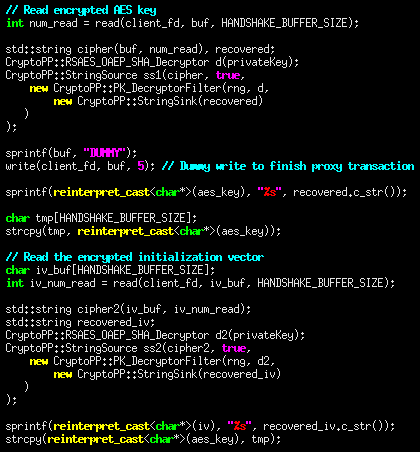
\includegraphics[height=0.8\textheight]{bankscreenshot_cropped.png}
\end{frame}

\begin{frame}[fragile]
\frametitle{RCE Attempt (Stack diagram)}
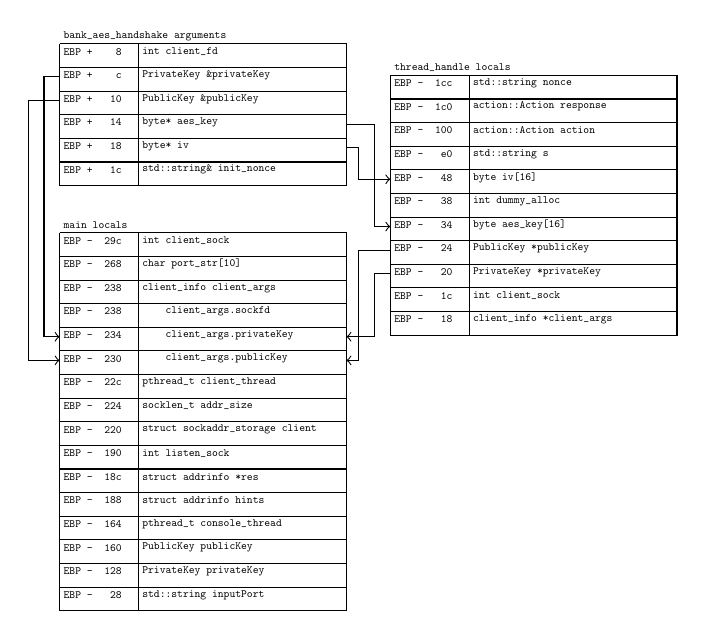
\begin{tikzpicture}[scale=0.4, every node/.style={scale=0.4}]
\draw (1.0,6.25) node[right]{\Verb|bank_aes_handshake arguments|};\draw (1.0,6.0) -- (10.1,6.0) -- (10.1,5.25) -- (1.0,5.25)-- (1.0,6.0);\draw (3.5,5.75) node[right]{\Verb|int client_fd|};\draw (1.0, 5.75) node[right]{\verb|EBP +    8|};\draw (3.5,6.0) -- (3.5, 5.25);\draw (1.0,5.25) -- (10.1,5.25) -- (10.1,4.5) -- (1.0,4.5)-- (1.0,5.25);\draw (3.5,5.0) node[right]{\Verb|PrivateKey &privateKey|};\draw (1.0, 5.0) node[right]{\verb|EBP +    c|};\draw (3.5,5.25) -- (3.5, 4.5);\draw (1.0,4.5) -- (10.1,4.5) -- (10.1,3.75) -- (1.0,3.75)-- (1.0,4.5);\draw (3.5,4.25) node[right]{\Verb|PublicKey &publicKey|};\draw (1.0, 4.25) node[right]{\verb|EBP +   10|};\draw (3.5,4.5) -- (3.5, 3.75);\draw (1.0,3.75) -- (10.1,3.75) -- (10.1,3.0) -- (1.0,3.0)-- (1.0,3.75);\draw (3.5,3.5) node[right]{\Verb|byte* aes_key|};\draw (1.0, 3.5) node[right]{\verb|EBP +   14|};\draw (3.5,3.75) -- (3.5, 3.0);\draw (1.0,3.0) -- (10.1,3.0) -- (10.1,2.25) -- (1.0,2.25)-- (1.0,3.0);\draw (3.5,2.75) node[right]{\Verb|byte* iv|};\draw (1.0, 2.75) node[right]{\verb|EBP +   18|};\draw (3.5,3.0) -- (3.5, 2.25);\draw (1.0,2.25) -- (10.1,2.25) -- (10.1,1.5) -- (1.0,1.5)-- (1.0,2.25);\draw (3.5,2.0) node[right]{\Verb|std::string& init_nonce|};\draw (1.0, 2.0) node[right]{\verb|EBP +   1c|};\draw (3.5,2.25) -- (3.5, 1.5);\draw (11.5,5.25) node[right]{\Verb|thread_handle locals|};\draw (11.5,5.0) -- (20.6,5.0) -- (20.6,4.25) -- (11.5,4.25)-- (11.5,5.0);\draw (14.0,4.75) node[right]{\Verb|std::string nonce|};\draw (11.5, 4.75) node[right]{\verb|EBP -  1cc|};\draw (14.0,5.0) -- (14.0, 4.25);\draw (11.5,4.25) -- (20.6,4.25) -- (20.6,3.5) -- (11.5,3.5)-- (11.5,4.25);\draw (14.0,4.0) node[right]{\Verb|action::Action response|};\draw (11.5, 4.0) node[right]{\verb|EBP -  1c0|};\draw (14.0,4.25) -- (14.0, 3.5);\draw (11.5,3.5) -- (20.6,3.5) -- (20.6,2.75) -- (11.5,2.75)-- (11.5,3.5);\draw (14.0,3.25) node[right]{\Verb|action::Action action|};\draw (11.5, 3.25) node[right]{\verb|EBP -  100|};\draw (14.0,3.5) -- (14.0, 2.75);\draw (11.5,2.75) -- (20.6,2.75) -- (20.6,2.0) -- (11.5,2.0)-- (11.5,2.75);\draw (14.0,2.5) node[right]{\Verb|std::string s|};\draw (11.5, 2.5) node[right]{\verb|EBP -   e0|};\draw (14.0,2.75) -- (14.0, 2.0);\draw (11.5,2.0) -- (20.6,2.0) -- (20.6,1.25) -- (11.5,1.25)-- (11.5,2.0);\draw (14.0,1.75) node[right]{\Verb|byte iv[16]|};\draw (11.5, 1.75) node[right]{\verb|EBP -   48|};\draw (14.0,2.0) -- (14.0, 1.25);\draw (11.5,1.25) -- (20.6,1.25) -- (20.6,0.5) -- (11.5,0.5)-- (11.5,1.25);\draw (14.0,1.0) node[right]{\Verb|int dummy_alloc|};\draw (11.5, 1.0) node[right]{\verb|EBP -   38|};\draw (14.0,1.25) -- (14.0, 0.5);\draw (11.5,0.5) -- (20.6,0.5) -- (20.6,-0.25) -- (11.5,-0.25)-- (11.5,0.5);\draw (14.0,0.25) node[right]{\Verb|byte aes_key[16]|};\draw (11.5, 0.25) node[right]{\verb|EBP -   34|};\draw (14.0,0.5) -- (14.0, -0.25);\draw (11.5,-0.25) -- (20.6,-0.25) -- (20.6,-1.0) -- (11.5,-1.0)-- (11.5,-0.25);\draw (14.0,-0.5) node[right]{\Verb|PublicKey *publicKey|};\draw (11.5, -0.5) node[right]{\verb|EBP -   24|};\draw (14.0,-0.25) -- (14.0, -1.0);\draw (11.5,-1.0) -- (20.6,-1.0) -- (20.6,-1.75) -- (11.5,-1.75)-- (11.5,-1.0);\draw (14.0,-1.25) node[right]{\Verb|PrivateKey *privateKey|};\draw (11.5, -1.25) node[right]{\verb|EBP -   20|};\draw (14.0,-1.0) -- (14.0, -1.75);\draw (11.5,-1.75) -- (20.6,-1.75) -- (20.6,-2.5) -- (11.5,-2.5)-- (11.5,-1.75);\draw (14.0,-2.0) node[right]{\Verb|int client_sock|};\draw (11.5, -2.0) node[right]{\verb|EBP -   1c|};\draw (14.0,-1.75) -- (14.0, -2.5);\draw (11.5,-2.5) -- (20.6,-2.5) -- (20.6,-3.25) -- (11.5,-3.25)-- (11.5,-2.5);\draw (14.0,-2.75) node[right]{\Verb|client_info *client_args|};\draw (11.5, -2.75) node[right]{\verb|EBP -   18|};\draw (14.0,-2.5) -- (14.0, -3.25);\draw (1.0,0.25) node[right]{\Verb|main locals|};\draw (1.0,0.0) -- (10.1,0.0) -- (10.1,-0.75) -- (1.0,-0.75)-- (1.0,0.0);\draw (3.5,-0.25) node[right]{\Verb|int client_sock|};\draw (1.0, -0.25) node[right]{\verb|EBP -  29c|};\draw (3.5,0.0) -- (3.5, -0.75);\draw (1.0,-0.75) -- (10.1,-0.75) -- (10.1,-1.5) -- (1.0,-1.5)-- (1.0,-0.75);\draw (3.5,-1.0) node[right]{\Verb|char port_str[10]|};\draw (1.0, -1.0) node[right]{\verb|EBP -  268|};\draw (3.5,-0.75) -- (3.5, -1.5);\draw (1.0,-1.5) -- (10.1,-1.5) -- (10.1,-2.25) -- (1.0,-2.25)-- (1.0,-1.5);\draw (3.5,-1.75) node[right]{\Verb|client_info client_args|};\draw (1.0, -1.75) node[right]{\verb|EBP -  238|};\draw (3.5,-1.5) -- (3.5, -2.25);\draw (1.0,-2.25) -- (10.1,-2.25) -- (10.1,-3.0) -- (1.0,-3.0)-- (1.0,-2.25);\draw (3.5,-2.5) node[right]{\Verb|    client_args.sockfd|};\draw (1.0, -2.5) node[right]{\verb|EBP -  238|};\draw (3.5,-2.25) -- (3.5, -3.0);\draw (1.0,-3.0) -- (10.1,-3.0) -- (10.1,-3.75) -- (1.0,-3.75)-- (1.0,-3.0);\draw (3.5,-3.25) node[right]{\Verb|    client_args.privateKey|};\draw (1.0, -3.25) node[right]{\verb|EBP -  234|};\draw (3.5,-3.0) -- (3.5, -3.75);\draw (1.0,-3.75) -- (10.1,-3.75) -- (10.1,-4.5) -- (1.0,-4.5)-- (1.0,-3.75);\draw (3.5,-4.0) node[right]{\Verb|    client_args.publicKey|};\draw (1.0, -4.0) node[right]{\verb|EBP -  230|};\draw (3.5,-3.75) -- (3.5, -4.5);\draw (1.0,-4.5) -- (10.1,-4.5) -- (10.1,-5.25) -- (1.0,-5.25)-- (1.0,-4.5);\draw (3.5,-4.75) node[right]{\Verb|pthread_t client_thread|};\draw (1.0, -4.75) node[right]{\verb|EBP -  22c|};\draw (3.5,-4.5) -- (3.5, -5.25);\draw (1.0,-5.25) -- (10.1,-5.25) -- (10.1,-6.0) -- (1.0,-6.0)-- (1.0,-5.25);\draw (3.5,-5.5) node[right]{\Verb|socklen_t addr_size|};\draw (1.0, -5.5) node[right]{\verb|EBP -  224|};\draw (3.5,-5.25) -- (3.5, -6.0);\draw (1.0,-6.0) -- (10.1,-6.0) -- (10.1,-6.75) -- (1.0,-6.75)-- (1.0,-6.0);\draw (3.5,-6.25) node[right]{\Verb|struct sockaddr_storage client|};\draw (1.0, -6.25) node[right]{\verb|EBP -  220|};\draw (3.5,-6.0) -- (3.5, -6.75);\draw (1.0,-6.75) -- (10.1,-6.75) -- (10.1,-7.5) -- (1.0,-7.5)-- (1.0,-6.75);\draw (3.5,-7.0) node[right]{\Verb|int listen_sock|};\draw (1.0, -7.0) node[right]{\verb|EBP -  190|};\draw (3.5,-6.75) -- (3.5, -7.5);\draw (1.0,-7.5) -- (10.1,-7.5) -- (10.1,-8.25) -- (1.0,-8.25)-- (1.0,-7.5);\draw (3.5,-7.75) node[right]{\Verb|struct addrinfo *res|};\draw (1.0, -7.75) node[right]{\verb|EBP -  18c|};\draw (3.5,-7.5) -- (3.5, -8.25);\draw (1.0,-8.25) -- (10.1,-8.25) -- (10.1,-9.0) -- (1.0,-9.0)-- (1.0,-8.25);\draw (3.5,-8.5) node[right]{\Verb|struct addrinfo hints|};\draw (1.0, -8.5) node[right]{\verb|EBP -  188|};\draw (3.5,-8.25) -- (3.5, -9.0);\draw (1.0,-9.0) -- (10.1,-9.0) -- (10.1,-9.75) -- (1.0,-9.75)-- (1.0,-9.0);\draw (3.5,-9.25) node[right]{\Verb|pthread_t console_thread|};\draw (1.0, -9.25) node[right]{\verb|EBP -  164|};\draw (3.5,-9.0) -- (3.5, -9.75);\draw (1.0,-9.75) -- (10.1,-9.75) -- (10.1,-10.5) -- (1.0,-10.5)-- (1.0,-9.75);\draw (3.5,-10.0) node[right]{\Verb|PublicKey publicKey|};\draw (1.0, -10.0) node[right]{\verb|EBP -  160|};\draw (3.5,-9.75) -- (3.5, -10.5);\draw (1.0,-10.5) -- (10.1,-10.5) -- (10.1,-11.25) -- (1.0,-11.25)-- (1.0,-10.5);\draw (3.5,-10.75) node[right]{\Verb|PrivateKey privateKey|};\draw (1.0, -10.75) node[right]{\verb|EBP -  128|};\draw (3.5,-10.5) -- (3.5, -11.25);\draw (1.0,-11.25) -- (10.1,-11.25) -- (10.1,-12.0) -- (1.0,-12.0)-- (1.0,-11.25);\draw (3.5,-11.5) node[right]{\Verb|std::string inputPort|};\draw (1.0, -11.5) node[right]{\verb|EBP -   28|};\draw (3.5,-11.25) -- (3.5, -12.0);\draw[->] (1,4.95) -- (0.5,4.95) -- (0.5,-3.3) -- (1,-3.3);\draw[->] (1,4.2) -- (0,4.2) -- (0,-4.05) -- (1,-4.05);\draw[->] (11.5,-1.3) -- (11.0,-1.3) -- (11.0,-3.3) -- (10.1,-3.3);\draw[->] (11.5,-0.55) -- (10.5,-0.55) -- (10.5,-4.05) -- (10.1,-4.05);\draw[->] (10.1,3.45) -- (11.0,3.45) -- (11.0,0.2) -- (11.5,0.2);\draw[->] (10.1,2.7) -- (10.5,2.7) -- (10.5,1.7) -- (11.5,1.7);
\end{tikzpicture}
\end{frame}
\end{document}
